\documentclass[conference]{IEEEtran}
\IEEEoverridecommandlockouts
\usepackage{cite}
\usepackage{amsmath,amssymb,amsfonts}
\usepackage{algorithmic}
\usepackage{graphicx}
\usepackage{textcomp}
\usepackage{xcolor}
\usepackage{listings}

\lstset{
    basicstyle=\ttfamily\scriptsize,
    breaklines=true,
    breakatwhitespace=false,
    frame=single,
    numbers=left,
    numberstyle=\tiny\color{gray},
    numbersep=5pt,
    showstringspaces=false,
    tabsize=2,
    backgroundcolor=\color{gray!5},
    rulecolor=\color{black!40},
    columns=flexible,
    keepspaces=true,
    commentstyle=\color{gray!70},
    keywordstyle=\color{blue!70}\bfseries,
    stringstyle=\color{orange!70},
}

\lstdefinelanguage{JSX}{
  keywords={import, export, default, from, const, let, var,
             function, return, if, else, async, await,
             true, false, null, undefined, class, extends, new},
  morestring=[b]",
  morestring=[b]',
  morestring=[b]`,
  morecomment=[l]{//},
  morecomment=[s]{/*}{*/},
}

\lstdefinelanguage{Python3}{
  keywords={from, import, def, return, if, else, elif,
             not, and, or, True, False, None,
             raise, class, async, await, with, as, for, in, pass},
  morestring=[b]",
  morestring=[b]',
  morecomment=[l]{\#},
}

\def\BibTeX{{\rm B\kern-.05em{\sc i\kern-.025em b}\kern-.08em
    T\kern-.1667em\lower.7ex\hbox{E}\kern-.125emX}}

\begin{document}

% ==================== COVER PAGE ====================
\begin{titlepage}
\centering
\vspace*{0.5cm}

{\bfseries\large Mata Kuliah Workshop Pemrograman Framework \par}
\vspace{0.3cm}
{\bfseries\Large LAPORAN E - GOVERNANCE \par}
\vspace{0.2cm}
{\bfseries\Large Sistem Pengajuan Subsidi Pupuk Kabupaten Mojokerto \par}

\vfill

\includegraphics[width=0.45\textwidth]{image1.png}
\vfill

{\normalsize
Dosen Pengampu: \par
\vspace{0.1cm}
Amma Liesvarastranta Haz, S.Tr.T., M.T. \par
\vspace{0.6cm}
Disusun Oleh: \par
\vspace{0.1cm}
Syarifatullah Ceva Efendy (312521002) \par
Selby Wafi Nurjuan (3125521018) \par
}

\vfill

{\bfseries\large PROGRAM STUDI D3 TEKNIK INFORMATIKA PSDKU LAMONGAN \par}
\vspace{0.1cm}
{\bfseries\large DEPARTEMEN TEKNIK INFORMATIKA DAN KOMPUTER \par}
\vspace{0.1cm}
{\bfseries\large POLITEKNIK ELEKTRONIKA NEGERI SURABAYA \par}
\vspace{0.1cm}
{\bfseries\large 2026 \par}
\vspace*{0.5cm}

\end{titlepage}
\clearpage

% ==================== BAB I ====================
\title{E-Pupuk: Sistem Pengajuan Subsidi Pupuk Kabupaten Mojokerto Berbasis Data Terbuka Pemerintah\\
\thanks{Laporan Progres Mata Kuliah Workshop Pemrograman Framework, D3 Teknik Informatika PSDKU Lamongan, PENS.}
}

\author{
\IEEEauthorblockN{Syarifatullah Ceva Efendy\IEEEauthorrefmark{1}, Selby Wafi Nurjuan\IEEEauthorrefmark{2}}
\IEEEauthorblockA{Program Studi D3 Teknik Informatika PSDKU Lamongan\\
Politeknik Elektronika Negeri Surabaya\\
Email: \IEEEauthorrefmark{1}312521002@student.pens.ac.id, \IEEEauthorrefmark{2}3125521018@student.pens.ac.id}
}

\maketitle

\begin{abstract}
Pengelolaan dan penyaluran pupuk bersubsidi merupakan aspek krusial dalam mendukung produktivitas sektor pertanian di Kabupaten Mojokerto. Namun, proses rekapitulasi data dan pengajuan manual yang belum terintegrasi sering menimbulkan kendala seperti keterlambatan informasi, kesalahan pencatatan, serta ketidaksesuaian alokasi kuota. Penelitian ini mengusulkan E-Pupuk, sebuah sistem informasi berbasis web yang mengintegrasikan pendataan petani, pemeriksaan kuota RDKK, verifikasi oleh Petugas Penyuluh Lapangan (PPL), pencatatan realisasi distribusi, hingga pemantauan oleh Dinas Pertanian. Dengan memanfaatkan data terbuka pemerintah (open data) sebagai acuan awal, E-Pupuk meningkatkan efisiensi administrasi, transparansi informasi, serta akurasi penyaluran pupuk bersubsidi agar lebih tepat sasaran.
\end{abstract}

\begin{IEEEkeywords}
e-Governance, E-Pupuk, Subsidi Pupuk, Open Data, RDKK, Kabupaten Mojokerto.
\end{IEEEkeywords}

\section{Pendahuluan}
\subsection{Latar Belakang}
Perkembangan teknologi informasi dan komunikasi mendorong transformasi tata kelola pemerintahan menuju \textit{e-Governance}. Perubahan ini menuntut pelayanan publik yang lebih transparan, efisien, dan akuntabel melalui pemanfaatan teknologi serta pengelolaan data secara terintegrasi. Salah satu penerapannya adalah pemanfaatan data terbuka pemerintah (\textit{open data}) sebagai sumber data yang dapat mendukung proses pelayanan publik secara aktif \cite{b1}.

Dalam sektor pertanian, pemerintah Kabupaten Mojokerto menyalurkan program pupuk bersubsidi untuk membantu petani menjaga produktivitas dan mengurangi biaya produksi. Alokasi pupuk subsidi mengacu pada Rencana Definitif Kebutuhan Kelompok (RDKK) yang disusun oleh kelompok tani dan diteruskan kepada Dinas Pertanian. Namun, proses pengelolaan dan rekapitulasi data yang masih belum terintegrasi dapat menyebabkan keterlambatan penyampaian informasi, kesalahan pencatatan, serta kesulitan dalam melakukan verifikasi pengajuan pupuk \cite{b2}.

Kondisi tersebut juga menyebabkan petani kesulitan memperoleh informasi mengenai sisa kuota kelompok dan status pengajuan mereka. Di sisi lain, Petugas Penyuluh Lapangan (PPL) membutuhkan waktu dalam melakukan verifikasi pengajuan, sedangkan pihak Dinas Pertanian memerlukan sistem yang dapat membantu memantau realisasi penyaluran pupuk secara lebih cepat dan terstruktur. Oleh karena itu, diperlukan sistem yang mampu mengintegrasikan proses pengajuan, verifikasi, distribusi, serta pemantauan data pupuk bersubsidi \cite{b3}.

Sebagai solusi, dikembangkan E-Pupuk -- Sistem Pengajuan Subsidi Pupuk Kabupaten Mojokerto, yaitu sistem berbasis web yang mengintegrasikan pendataan petani dan lahan, pengajuan pupuk, pemeriksaan kuota RDKK, verifikasi oleh PPL, pencatatan realisasi distribusi, serta penyusunan laporan. Sistem ini diharapkan dapat meningkatkan efisiensi proses administrasi, mengurangi kesalahan data, meningkatkan transparansi informasi, dan membantu mewujudkan distribusi pupuk bersubsidi yang lebih tepat sasaran di Kabupaten Mojokerto \cite{b4}.

\subsection{Rumusan Masalah}
\begin{enumerate}
    \item Bagaimana mengelola data petani dan kelompok tani penerima pupuk subsidi secara terpusat?
    \item Bagaimana menentukan kewajaran kuota pengajuan pupuk berdasarkan data RDKK?
    \item Bagaimana membantu petugas penyuluh melakukan verifikasi pengajuan secara cepat dan objektif?
    \item Bagaimana petani dapat mengetahui status pengajuan dan distribusi pupuknya?
    \item Bagaimana Dinas Pertanian dapat memantau realisasi distribusi pupuk subsidi secara cepat dan terstruktur?
\end{enumerate}

\subsection{Tujuan}
\begin{enumerate}
    \item Membuat sistem pengelolaan data petani dan kelompok tani secara terintegrasi.
    \item Membantu proses verifikasi pengajuan berdasarkan data RDKK dan luas lahan.
    \item Mempermudah petani memperoleh informasi status pengajuan dan distribusi pupuk.
    \item Menyediakan dashboard monitoring dan pelaporan bagi Dinas Pertanian.
\end{enumerate}

\section*{Acknowledgment}
Penulis menyampaikan terima kasih kepada Dosen Pengampu Mata Kuliah Workshop Pemrograman Framework, Bapak Amma Liesvarastranta Haz, S.Tr.T., M.T., atas bimbingan dan arahan selama penyusunan laporan ini, serta Politeknik Elektronika Negeri Surabaya.

\begin{thebibliography}{00}
\bibitem{b1} R. Heeks, ``Implementing and Managing e-Government: An International Text,'' SAGE Publications, 2006.
\bibitem{b2} Kementerian Pertanian Republik Indonesia, ``Pedoman Pengelolaan Sistem Elektronik Rencana Definitif Kebutuhan Kelompok (e-RDKK),'' Jakarta, 2021.
\bibitem{b3} Dinas Pertanian Kabupaten Mojokerto, ``Laporan Evaluasi Penyaluran Pupuk Bersubsidi Kabupaten Mojokerto,'' 2024.
\bibitem{b4} A. S. Ahmad, ``Pemanfaatan Open Government Data untuk Transparansi Layanan Publik di Sektor Pertanian,'' Jurnal Teknologi dan Governance, vol. 8, no. 1, pp. 45--56, 2023.
\end{thebibliography}

% ==================== PERALIHAN KE 1 KOLOM ====================
\clearpage
\onecolumn

% ==================== BAB II: SUMBER KODE ====================
\section{Sumber Kode}
\label{sec:sumber_kode}

%-------- 2.1 Frontend App.jsx --------
\subsection{Frontend --- \texttt{App.jsx}}
\lstinputlisting[language=JSX, caption={frontend/src/App.jsx}]{frontend/src/App.jsx}

\clearpage

%-------- 2.2 Backend main.py --------
\subsection{Backend --- \texttt{main.py}}
\lstinputlisting[language=Python3, caption={backend/app/main.py}]{backend/app/main.py}

\clearpage

%-------- 2.3 Backend auth.py --------
\subsection{Backend --- \texttt{routers/auth.py}}
\lstinputlisting[language=Python3, caption={backend/app/routers/auth.py}]{backend/app/routers/auth.py}

\clearpage

%-------- 2.4 Backend applications.py --------
\subsection{Backend --- \texttt{routers/applications.py}}
\lstinputlisting[language=Python3, caption={backend/app/routers/applications.py}]{backend/app/routers/applications.py}

\clearpage

%-------- 2.5 Backend ppl.py --------
\subsection{Backend --- \texttt{routers/ppl.py}}
\lstinputlisting[language=Python3, caption={backend/app/routers/ppl.py}]{backend/app/routers/ppl.py}

\clearpage

%-------- 2.6 Backend admin.py --------
\subsection{Backend --- \texttt{routers/admin.py}}
\lstinputlisting[language=Python3, caption={backend/app/routers/admin.py}]{backend/app/routers/admin.py}

\clearpage

%-------- 2.7 Database schema.sql --------
\subsection{Database --- \texttt{schema.sql}}
\lstinputlisting[language=SQL, caption={backend/schema.sql}]{backend/schema.sql}


\clearpage


% ==================== BAB III ====================
\section{Design System}
\label{sec:design_system}

Design system E-Pupuk merancang visual konsisten, komponen antarmuka modular, skema warna yang harmonis, dan elemen navigasi intuitif untuk pengguna dari berbagai peran (Petani, PPL, Admin, dan Pimpinan Dinas).

\begin{figure}[htbp]
    \centering
    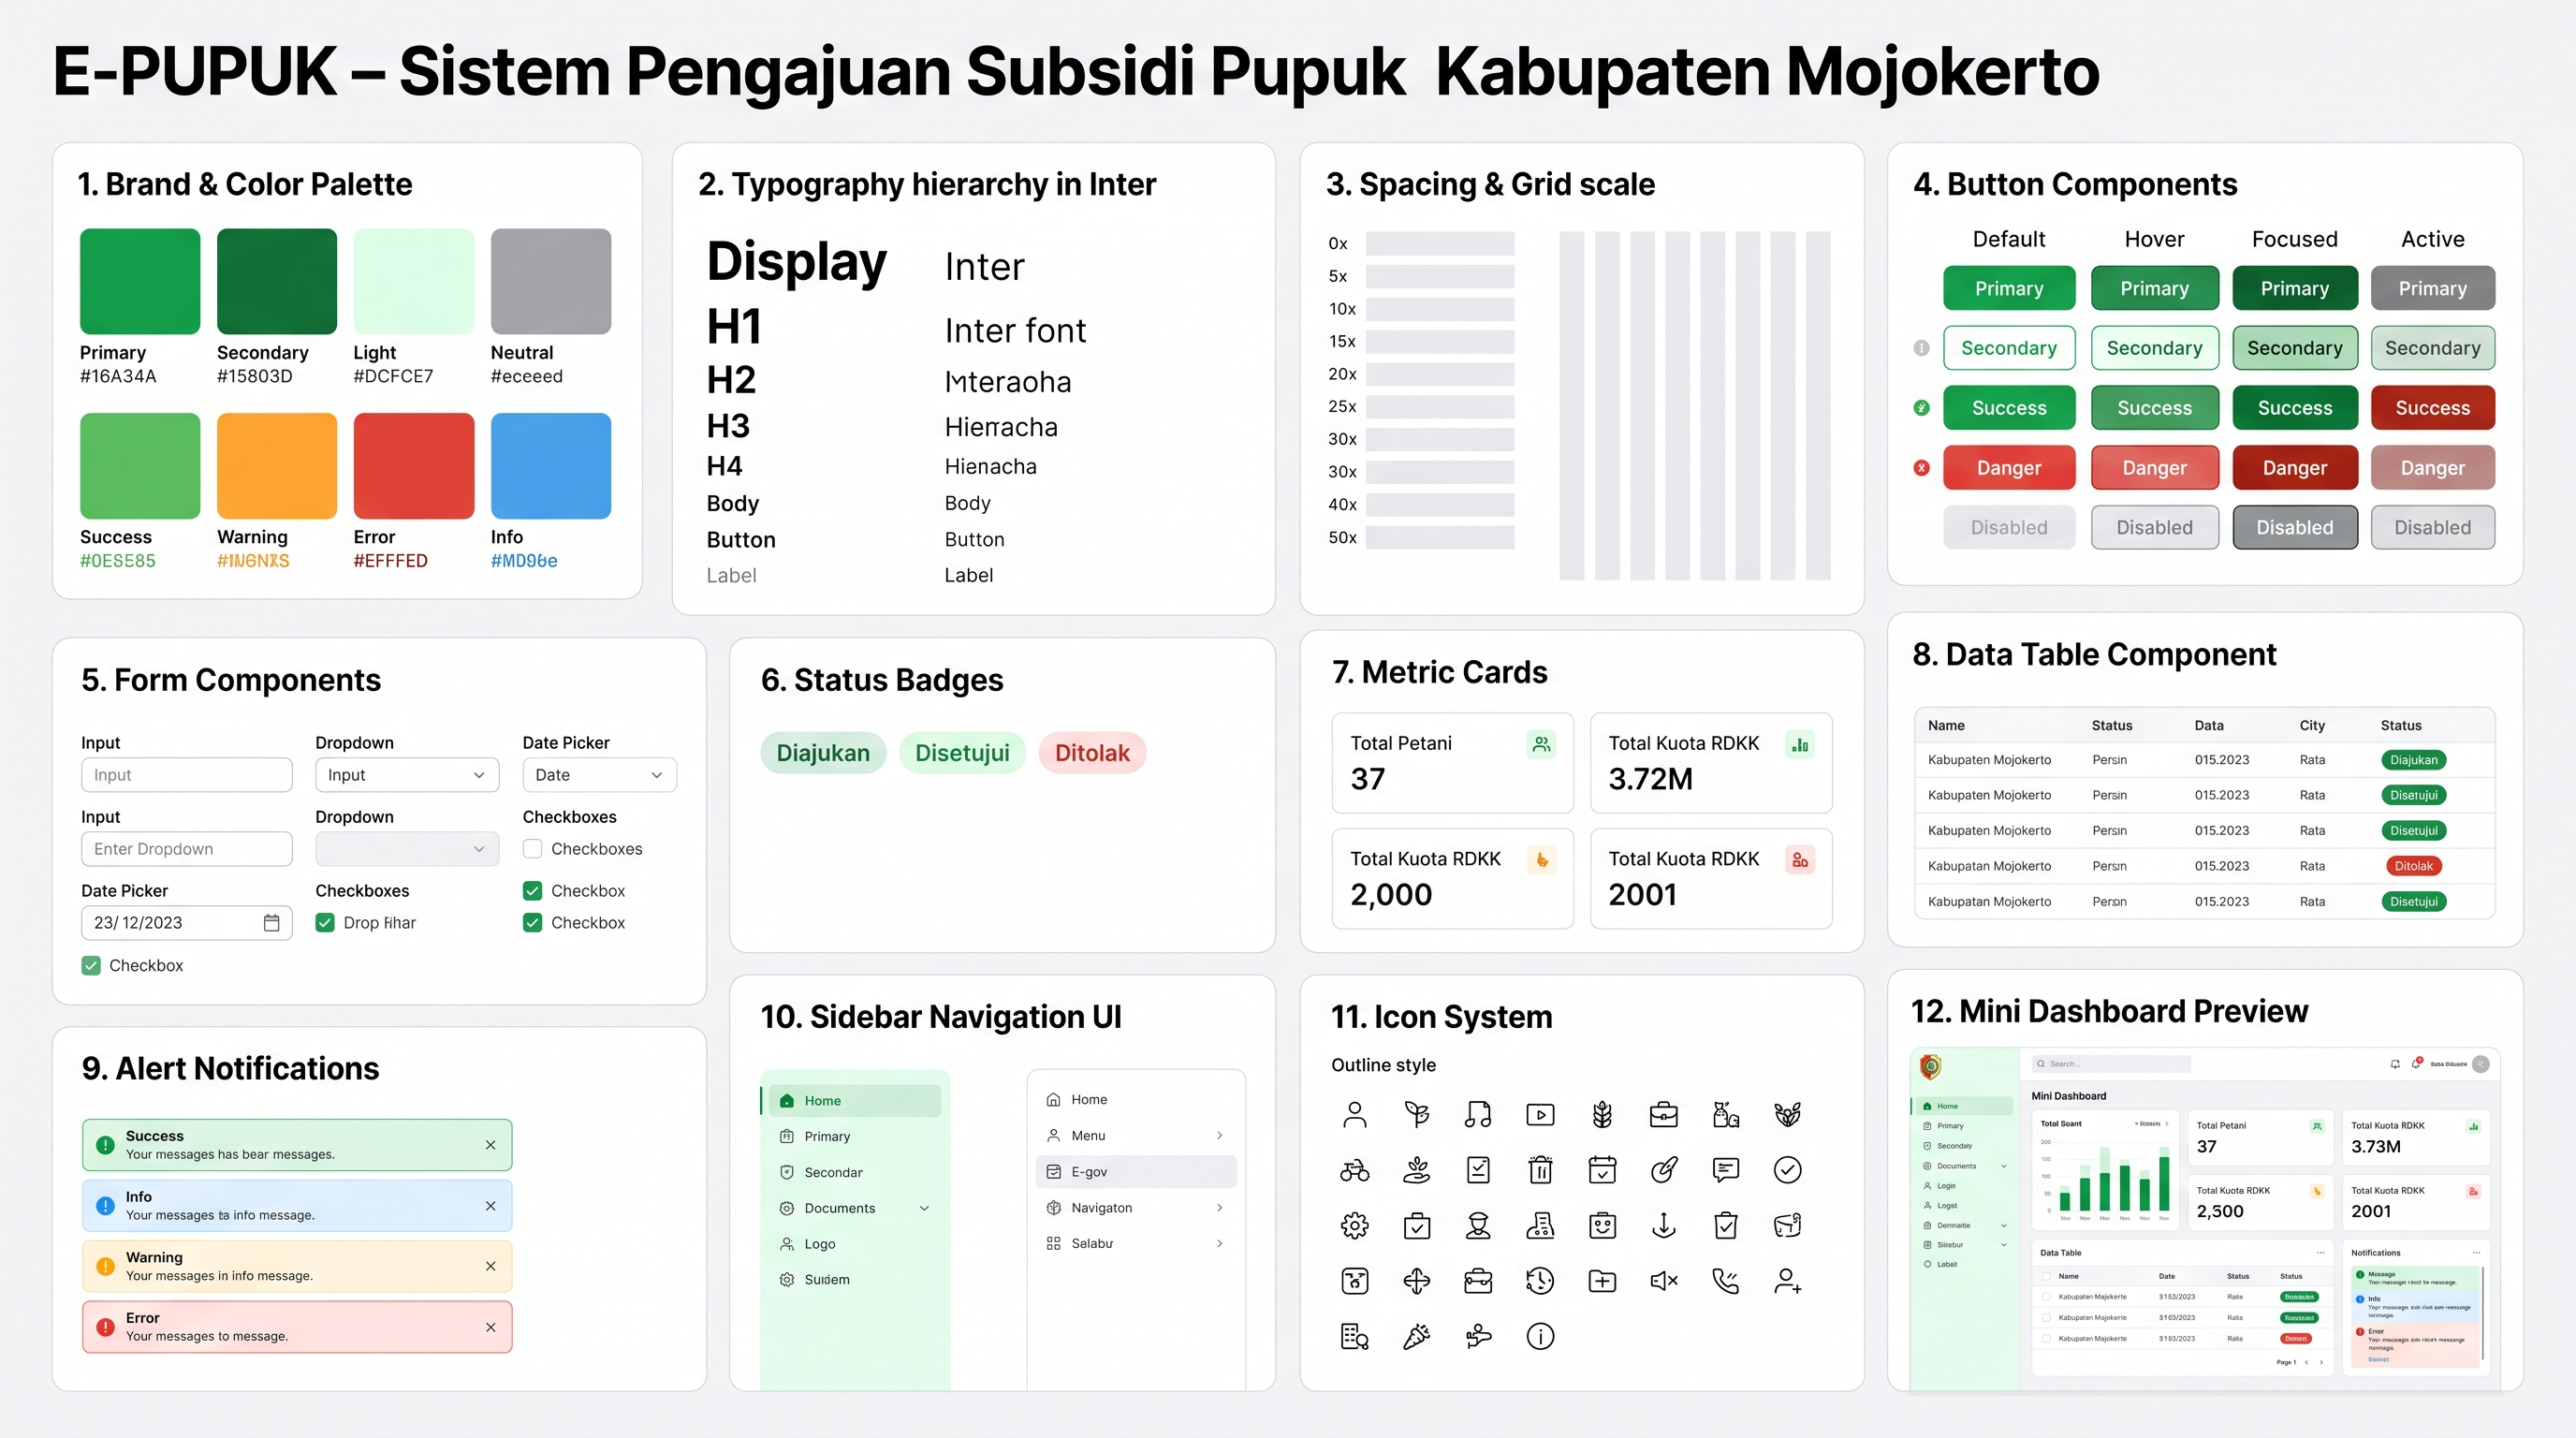
\includegraphics[width=0.9\textwidth]{design system.png}
    \caption{Design System E-Pupuk}
    \label{fig:design_system}
\end{figure}

\clearpage

% ==================== BAB IV ====================
\section{Arsitektur sistem}
\label{sec:arsitektur_sistem}

Arsitektur sistem E-Pupuk mengintegrasikan komponen frontend (React Web App), backend REST API (Python FastAPI), serta basis data terpusat (MySQL). Data terbuka pemerintah dimanfaatkan melalui modul data-seeding untuk memberikan informasi baseline kuota RDKK dan luas lahan.

\begin{figure}[htbp]
    \centering
    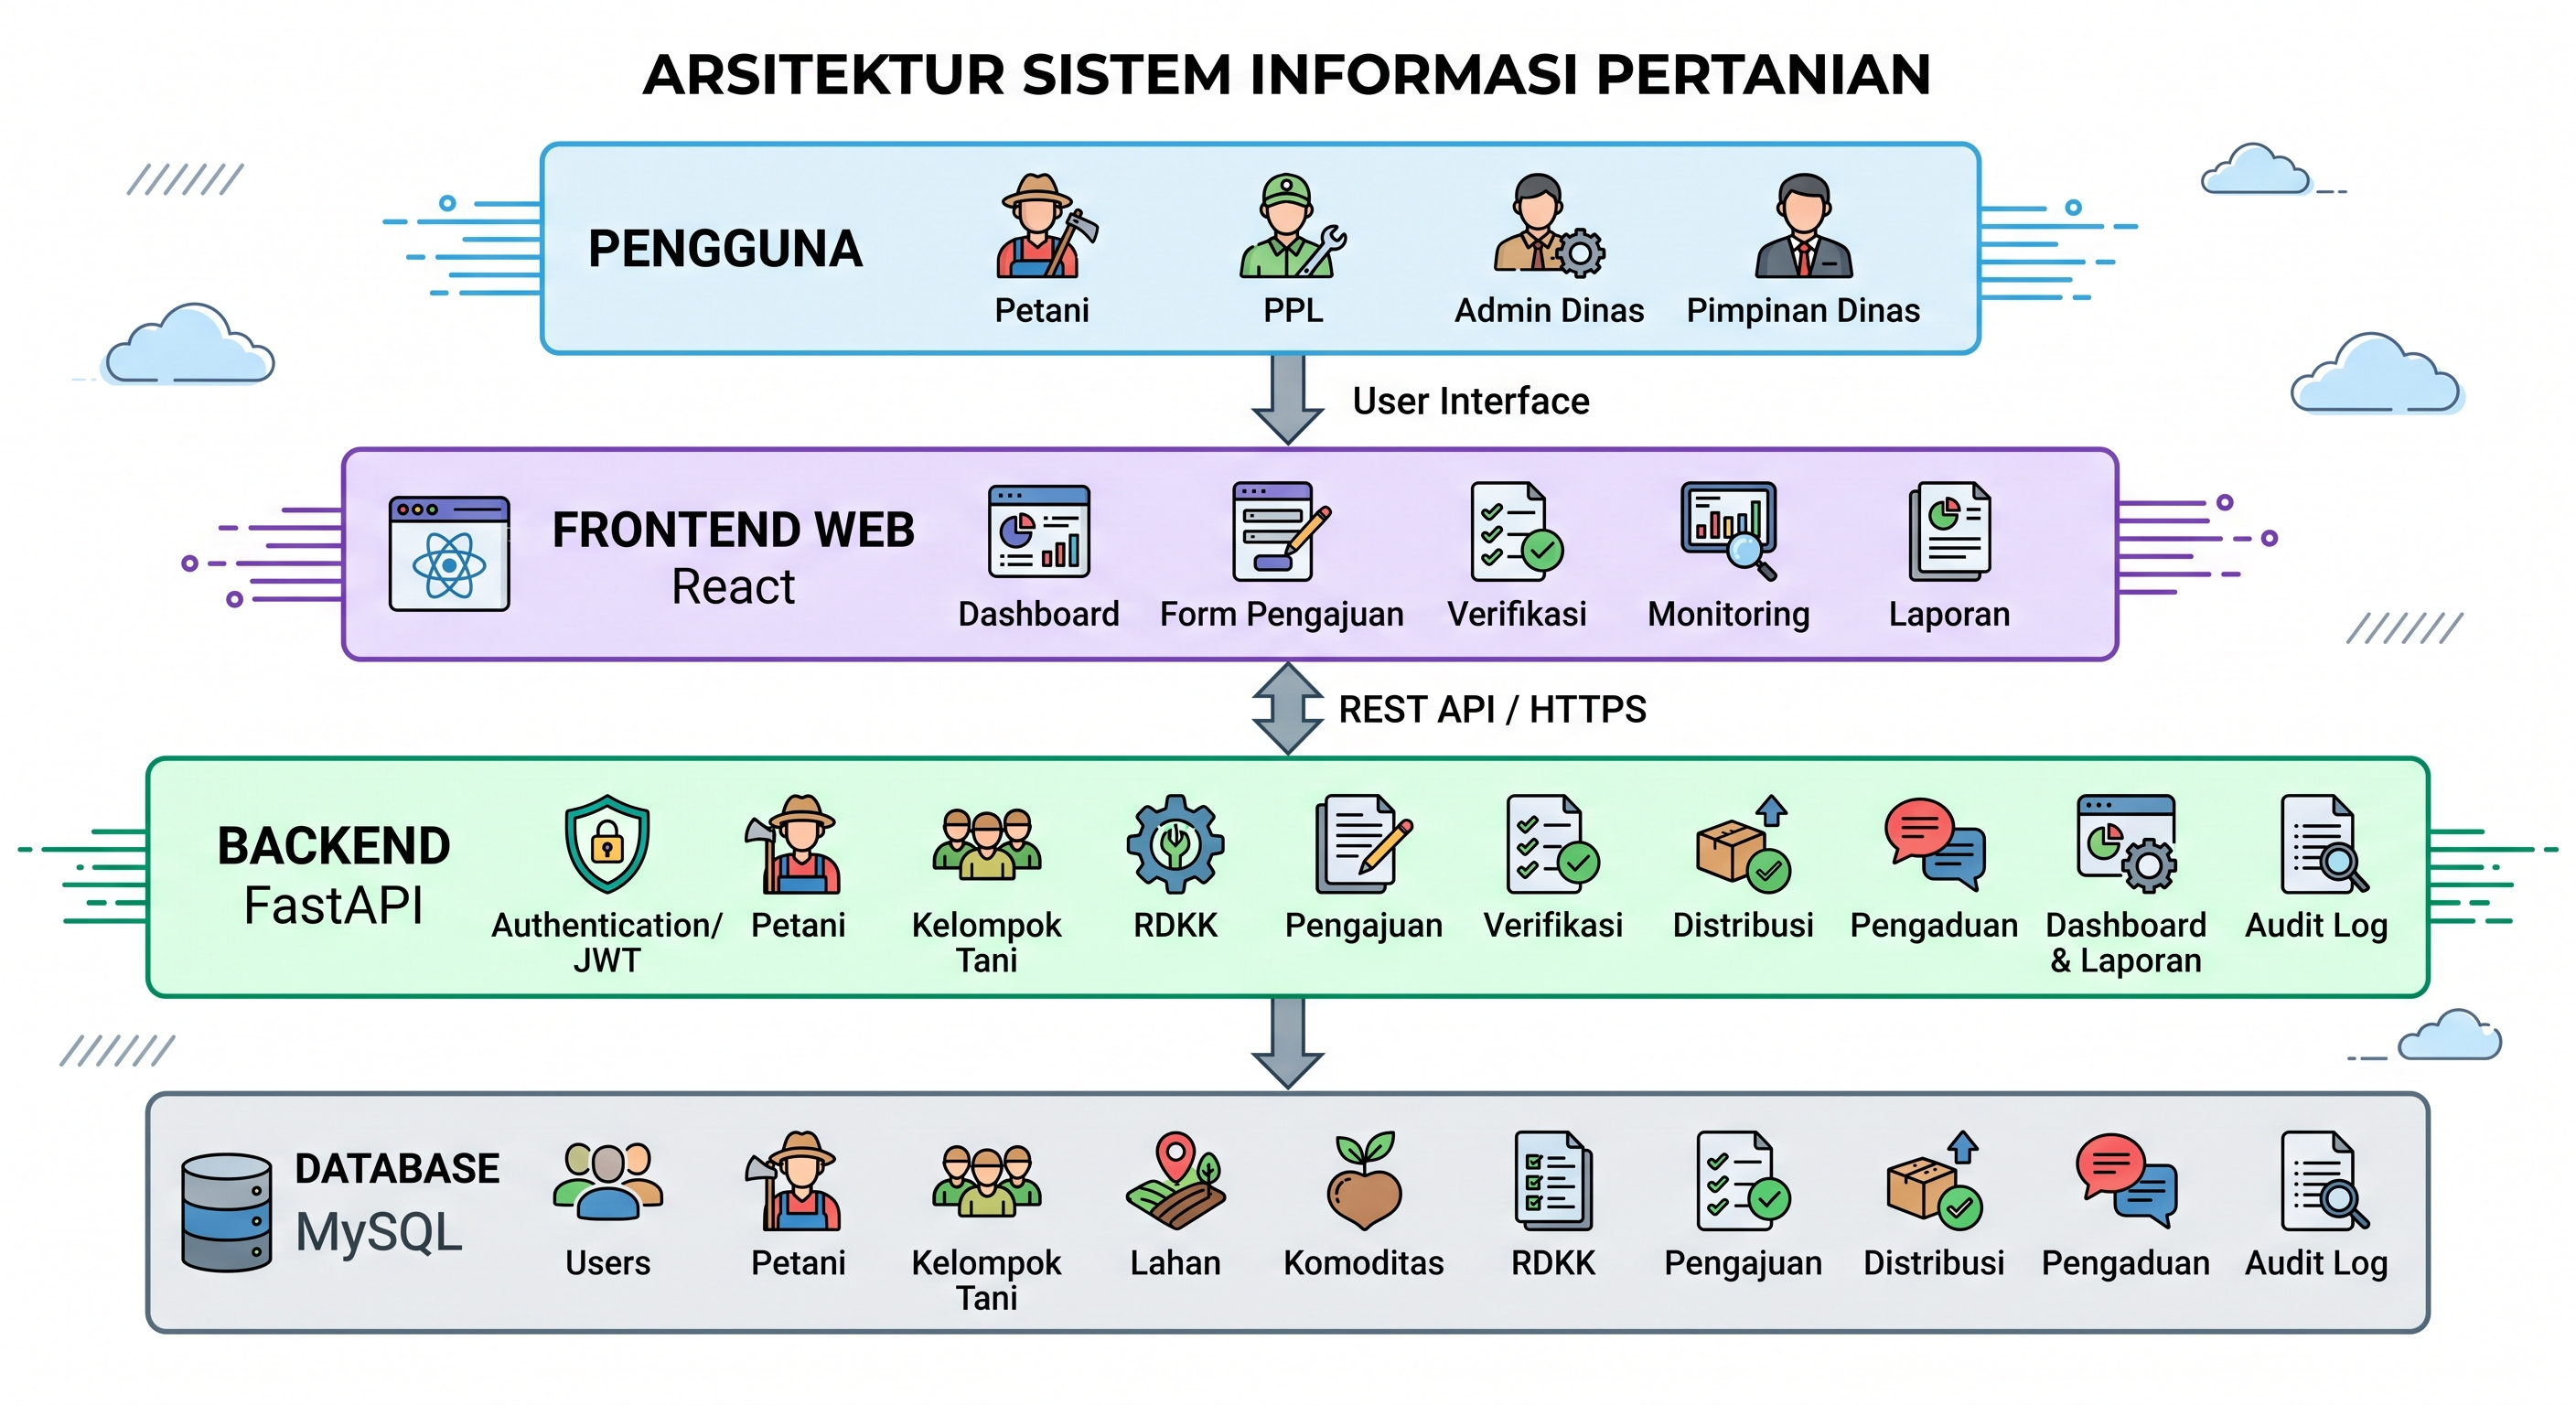
\includegraphics[width=0.9\textwidth]{arsitektur sistem.png}
    \caption{Arsitektur Sistem E-Pupuk}
    \label{fig:architecture_system}
\end{figure}

\clearpage

% ==================== BAB V ====================
\section{Mockup UI}
\label{sec:mockup_ui}

Bab ini menyajikan 5 rancangan antarmuka (\textit{Mockup UI}) utama sistem E-Pupuk dari folder \textit{Frontend} yang mencakup alur proses pengguna dari halaman utama, pengajuan petani, verifikasi PPL, hingga monitoring eksekutif Dinas Pertanian.

\begin{figure}[htbp]
    \centering
    
\includegraphics[width=0.85\textwidth,height=0.65\textheight,keepaspectratio]{{Image/Beranda E-Pupuk Mojokerto - Agri-Gov Blue}.png}
    \caption{Mockup UI -- Halaman Utama / Beranda E-Pupuk Kabupaten Mojokerto}
    \label{fig:mockup_beranda}
\end{figure}

\clearpage

\begin{figure}[htbp]
    \centering
    
\includegraphics[width=0.85\textwidth,height=0.65\textheight,keepaspectratio]{{Image/Dashboard Petani - Agri-Gov Blue}.png}
    \caption{Mockup UI -- Dashboard Petani (Informasi Kuota RDKK dan Status Lahan)}
    \label{fig:mockup_dashboard_petani}
\end{figure}

\clearpage

\begin{figure}[htbp]
    \centering
    
\includegraphics[width=0.85\textwidth,height=0.65\textheight,keepaspectratio]{{Image/Ajukan Kebutuhan Pupuk - Agri-Gov Blue}.png}
    \caption{Mockup UI -- Form Pengajuan Kebutuhan Pupuk Subsidi oleh Petani}
    \label{fig:mockup_pengajuan}
\end{figure}

\clearpage

\begin{figure}[htbp]
    \centering
    
\includegraphics[width=0.85\textwidth,height=0.65\textheight,keepaspectratio]{{Image/Detail Verifikasi Pengajuan - PPL Mojokerto}.png}
    \caption{Mockup UI -- Halaman Verifikasi Pengajuan Pupuk oleh Petugas Penyuluh Lapangan (PPL)}
    \label{fig:mockup_verifikasi_ppl}
\end{figure}

\clearpage

\begin{figure}[htbp]
    \centering
    
\includegraphics[width=0.85\textwidth,height=0.65\textheight,keepaspectratio]{{Image/Dashboard Monitoring Eksekutif - E-Pupuk Mojokerto}.png}
    \caption{Mockup UI -- Dashboard Monitoring Eksekutif Dinas Pertanian}
    \label{fig:mockup_dashboard_eksekutif}
\end{figure}

\end{document}
